\documentclass[12pt, a4paper]{article}
\usepackage[utf8]{inputenc}
\usepackage[IL2]{fontenc}
\usepackage[czech]{babel}
\usepackage{graphicx}
\usepackage{footnote}
\usepackage{fancyvrb}

\begin{document}
\begin{figure}[h!]
\centering

\includegraphics[bb= 0 0 820 445 , width=75mm]{favlogo.jpg}
\end{figure}

{\centering
{\huge Systém automatické indexace}\\[1em]
{\large KIV/IR}\\[11,5cm]
}

\begin{tabular}{l r}
student: & Radek VAIS\\
os. číslo: & A17N0093P\\
mail: & vaisr@students.zcu.cz\\
datum: & 23.5.2018\\
\end{tabular}

\thispagestyle{empty}
\newpage

%========================================
%========================================
%========================================
%========================================
%========================================
\section{Zadání} %=====================================================================================================

S využitím připravených rozhraní v jazyce Java navrhněte a implementujte systém automatické indexace a vyhledávání dokumentů.

\subsection{Minimální funkčnost:}

Tokenizace, Preprocessing (stopwords remover, stemmer/lemmatizer), vytvoření in-memory invertovaného indexu, tf-idf model, cosine similarity,  vyhledávání pomocí dotazu vrací top x výsledků seřazených dle relevance, vyhledávání s pomocí logických operátorů AND, OR, NOT, podrobná dokumentace (programátorská i uživatelská)

\subsection{Nadstandardní funkčnost:}

File-based index (1b), pozdější doindexování dat (1b), ošetření např. HTML tagů (1b), detekce jazyka (1b), vylepšení vyhledávání (1b), vyhledávání frází (i stop slova)(1b), vyhledávání v okolí slova (1b), více scoring modelů (1b),  indexování webového obsahu (2b), další předzpracování normalizace (1b), webové rozhraní/GUI (2b), napovídání keywords (1b), podpora více polí pro dokument (např. datum)(1b), CRUD indexovaných dokumentů (2b), zvýraznění hledaného textu v náhledu výsledků (1b), dokumentace psaná v TEXu (1b), atd. (xb)


%====================================================================================================================================================
\newpage

\section{Analýza zadání}

\subsection{Invertovaný index}

Invertovaný index je datová struktura, která slouží pro snadné vyhledávání v dokumentech. Jedná se o mapu, kde klíčem je term, na který je navázaný seznam výskytů v dokumentech. Při použití různých kompresních optimalizací lze oddělit slovník termů od indexu samotného. Případně lze strukturu výskytu dokumentu obohatit o četnost výskytu termu v dokumentu. Pro potřeby semestrální práce dostačuje použít nekomprimovanou verzi indexu. Index tedy může vypadat následujícím způsobem:

\begin{figure}[ht!]
\centering
\begin{BVerbatim}
index:
    term:
        doc1: 3
        doc3: 4
    term1:
        doc2: 1
        doc3: 4
\end{BVerbatim}
\end{figure}


\subsection{Metrika TF-IDF}

Metrika TF-IDF je kompozicí dvou metrik. První metrikou je TF, tedy zhodnocení počtu výskytu daného termu v dokumentu, jejíž hodnotu získáme následujícím způsobem:

\begin{equation}
w(t,d) = \left\{ \begin{array}{r@{\quad}c}
    1 + \log_{10}(tf_{t,d}), & {tf}_{t,d} > 0 \\
    0, & {tf}_{t,d} = 0 \\ \end{array} \right.
\end{equation}
,kde $tf_{t,d}$ je počet výskytů termu $t$ v dokumentu $d$.

Druhou metrikou je IDF, která popisuje jak častý je term v celé kolekci dokumentů její hodnotu získáme následujícím způsobem:

\begin{equation}
idf(t) = \log_{10}\frac{N}{df_{t}}
\end{equation}
,kde $N$ je celkový počet indexovaných dokumentů $df_{t}$ je počet dokumentů obsahující term $t$.


Výsledná kompozice metrik je následující:

\begin{equation}
tfidf(t,d) = (1 + log_{10}tf_{t,d}) \cdot \log_{10}\frac{N}{df_{t}}
\end{equation}


\subsection{Cosinová podobnost}

Pro vyhodnocení nejlepšího dokumentu lze využít metriku cosinové podobnosti. Pro tuto metriku je třeba definovat vektorovou reprezentaci dokumentů a dotazů. Vektor reprezentující dokument bude tvořen hodnotami \emph{tf-idf} pro jednotlivé termy dokumentu. Cosinová podobnost se vypčítá následujícím způsobem:

\begin{equation}
\label{eq:sim}
 similarity(\vec{A}, \vec{B}) = cos(\theta) = \frac{\vec{A} \cdot \vec{B}}{\parallel\vec{A}\parallel\parallel\vec{B}\parallel} 
\end{equation}

Ve výpočtu \ref{eq:sim} je použita kvadratická norma vektoru:
\begin{equation}
 norm(\vec{A}) = \parallel\vec{A}\parallel = \sqrt{\sum_{i=1} A_{i}^{2}} 
\end{equation}

\subsection{Booleovský dotaz}

Booleovský dotaz slouží k omezení seznamu vyhledávaných dokumentů. Dotaz může vypadat následujícím způsobem:
\begin{verbatim}
Petr AND Pavel AND NOT klíče OR automechanik
\end{verbatim} 
K parsování dotazu lze využít již existujících nástrojů např. \emph{Lucene} nebo \emph{AntLR}\footnote{Nástroj pro parsování textu dle gramatiky.} . Pro potřeby této semestrální práce není nezbytné využívat těchto velkých knihoven. Za předpokladu, že v dotazu nebudou použity závorky, je možné dotaz jednoduše rozdělit do větví dle OR a AND klíčových slov. Pro dotaz z příkladu pak vznikne následující derivační strom:

\begin{figure}[h!]
\centering
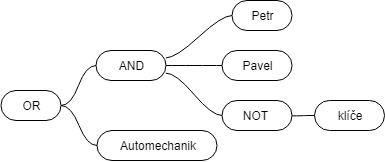
\includegraphics[bb= 0 0 385 162 , width=80mm]{boolean.png}
\label{fig:boolean}
\caption{Derivační strom ukázkového dotazu.}
\end{figure}

K implementaci průchodu takovým dotazem postačuje jednoduché dělení řetězců dle klíčových slov a korektní slučování výsledků dle žádané operace. Zpracování dotazu probíhá pre-order průchodem derivačním stromem.

%====================================================================================================================================================
\newpage
\section{Popis řešení}

Základní částí výsledného programového řešení je předzpracování dokumentu, a indexace. Pro předzpracování dokumentu bylo navrženo rozhraní \emph{IPreprocessor}, které z předaného textu vytvoří seznam tokenů. Instance předzpracování se předá třídě Index, která ji využívá pro předzpracování dokumentů a dotazů. Rozhraní \emph{IPreprocessor} je závislé na rozhraních \emph{ITokenizer} a IStemmer. ITokenizer poskytuje službu rozdělení textu na tokeny. \emph{IStemmer} posyktuje službu ořezání koncovek slov. Implementace tokenizéru \emph{BasicTokenizer} využívá rozhraní \emph{IDictionary} k realizaci slovníku stop slov. Vztahy mezi třídami jsou znázorněny na Obrázku \ref{fig:preprocessUML}.

\begin{figure}[h!]
\centering
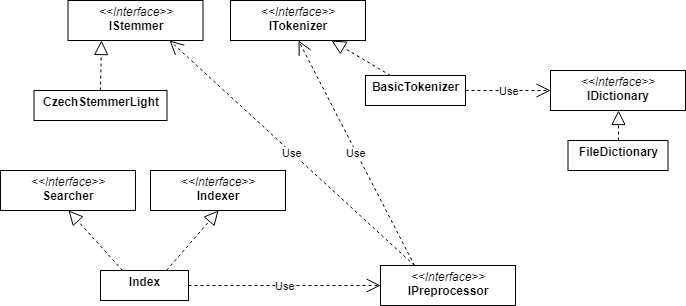
\includegraphics[bb= 0 0 686 306 , width=140mm]{UML-preprocess.png}
\label{fig:preprocessUML}
\caption{UML Diagram vztahů tříd preprocessingu.}
\end{figure}

Třída \emph{Index} interně uchovává mapu instancí třídy \emph{TokenProperties}, která slouží k uchování informace o nalezeném tokenu. Konkrétně je uchováván přesný text tokenu, mapa počtu výskytů v dokumentech (klíčem je ID dokumentu). Index také uchovává seznam index tokenů dle ID dokumentu, který slouží ke zrychlení vyhodnocení vyhledávání. Pro zvolený dokument se vyhodnocují hodnoty \emph{tf-idf} jen pro tokeny, které obsahuje.

Vyhodnocení vyhledávání je odpovědností tříd \emph{Evaluator} a \emph{DocumentVector}. Třída \emph{Evaluator} obsahuje metody pro výpočet vektoru \emph{tf-idf} pro dokument nebo dotaz. Třída \emph{DokumentVector} slouží jako reprezentace vektoru dokumentu, základní vlastností této třídy je výpočet cosinové podobnosti s jinými instancemi.    

Všechny komponenty uživatelského rozhraní jsou uloženy v balíku GUI. Pro implementaci je použita knihovna JavaFX a popisný XML formát FXML. 

\section{Ovládání}

\subsection{Sestavení}

Pro snadné sestavení a stažení závislostí je vhodné použit systém \texttt{maven}. Úkol \texttt{package} programu \texttt{maven} vytvoří ve složce \texttt{targets} dva spustitelné .jar archivy. Archiv \texttt{vaisr-Indexer.jar} ke svému běhu potřebuje zkopírovat složku \texttt{libs} obsahující závislé knihovny. Pro sestavení programu je třeba kompilátor jazyka Java ve verzi 8 a vyšší (závoslos na JavaFX). Program je dále závislý na knihovně Log4J (verze 2.11) a automatické testy části programu jsou implementovány pomocí knihovny JUnit (verze 5). Druhý archiv (\texttt{vaisr-Indexer-with-dependencies.jar}) obsahuje knihovny pro běh programu (Log4J) a je tedy samostatně přenositelný.

Závislosti sestavení:
\begin{itemize}
\item Java - verze 8

\item JavaFX - součást jazyka Java od verze 8.
\item Log4J - verze 2.11

\item JUnit - verze 5  \footnotemark[1]

\item Maven \footnotemark[1]

\footnotetext[1]{Doporučené programové vybavení.}

\end{itemize}

\subsection{Spuštění}

Výsledný \texttt{.jar} archiv lze spustit s následujícími parametry:

\begin{table}[ht!]
\centering
\begin{tabular}{l | l}
parametr & efekt\\
\hline
-eval   & Spustí větev kódu TestTrecEval\\
-small  & Bude indexován pouze název dokumentu.\\
-gui    & Po načtení indexu bude spuštěno GUI\\
-noLoad & Program se nepokusí nahrát uložený index.\\
-noSave & Program nebude ukládat vytvořený index.\\
-index [filePattern] & Slouží pro zadání cesty k a názvu indexu.\\
\end{tabular}
\end{table}

Při spuštění bez parametrů, se vypíše tato nápověda. Parametr \texttt{-eval} vylučuje použití parametru \texttt{-gui}. Parametr index očekává zadání cesty k a názvu indexu např. \emph{C:/xxx/index} program pak hledá ve složce \emph{C:/xxx} soubory pro načtení indexu s názvem \emph{index} analogicky se program chová pro ukládání. Případná chyba je zalogována na konzoli a do souboru.

Program očekává, že vstupní data budou uložena ve složce \texttt{TREC}, která leží v kořeni spuštění programu (standardně ve stejném umístění jako spouštěný \texttt{.jar}. Složka musí obsahovat datové soubory \texttt{czechData.bin}, pro vytváření indexu a \texttt{topicData.bin} pro evaluaci.

\subsubsection{Logování a výstup}

Program za běhu zaznamenává svoji činnost do několika souborů ve složce \texttt{log}. 
\begin{itemize}
\item VaisrEngine.log - obsahuje důležité záznamy o běhu vyhledávacího jádra.
\item VaisrEngine-GUI.log - obsahuje logové záznamy GUI.
\item VaisrEngine-dump.log - obsahuje všechny logové záznamy všech úrovní.
\end{itemize}

Při spuštění TestTrecEval program loguje výstup do složky \texttt{TREC} s názvem odpovídajícímu formátu \texttt{yyyy-MM-dd\_HH\_mm\_SS.log}. Dále je zde vytvořen soubor s výsledky vyhledávání.

\subsubsection{Grafické rozhraní}

Obrázek ...
Zadávání Booleovských dotazů .. neumí závorky

\section{Závěr}

V rámci této semestrální práce byl vytvořen systém automatické indexace a vyhledávání dokumentů s následujícími vlastnostmi funkcionalitou.

\begin{itemize}
\item Předzpracování
	\begin{itemize}
		\item Odstranění diakritiky
		\item Stemming slov
		\item Přeskočení stop slov.
		\item Tokenizace pomocí regulárních výrazů.
	\end{itemize}
\item{Indexace}
		\begin{itemize}
		\item Vytváření in-memory invertovaného indexu.
		\item Načítání indexu do paměti z uloženého souboru. (+1 bod)
		\item Možnost vytvářet index z názvu dokumentu nebo názvu a těla.
	\end{itemize}
\item{Vyhledávání}
	\begin{itemize}
		\item Vyhledávání pomocí booleovských operátorů.
		\item TF-IDF model.
		\item Cosinová podobnost.
	\end{itemize}
\item{Uživatelské rozhraní}
	\begin{itemize}
		\item Implementováno pomocí prostředků JavaFX (+2 body)
		\item Možnost zadat dotaz.
		\item Zobrazení top 10 výsledků.
		\item Možnost načtení uloženého indexu.
	\end{itemize}
\item{Dokumentace}
	\begin{itemize}
		\item Akademická dokumentace sázena systémem \LaTeX (+1 bod)
		\item Uživatelská dokumentace. (součást akademické)
		\item Programátorská dokumentace JavaDoc. (součást odevzdávaného archivu) 
	\end{itemize}	
\end{itemize}

Výsledky dosažené pomocí evaluátoru:

\begin{verbatim}
TODO kopie výsledků
\end{verbatim}

\end{document}